 % -*- TeX-engine: xetex; eval: (auto-fill-mode 0); eval: (visual-line-mode 1); -*-
% Compile with XeLaTeX

%%%%%%%%%%%%%%%%%%%%%%%
% To do before class
%%%%%%%%%%%%%%%%%%%%%%%

% Print off Readiness Assessment 1.
% Send email about registering clicker.
% Test run readiness assessment on iClicker.

%%%%%%%%%%%%%%%%%%%%%%%
% Option 1: Slides: (comment for handouts)   %
%%%%%%%%%%%%%%%%%%%%%%%

%\documentclass[slidestop,compress,mathserif,12pt,t,professionalfonts,xcolor=table]{beamer}
%
%% solution stuff
%\newcommand{\solnMult}[1]{
%\only<1>{#1}
%\only<2->{\red{\textbf{#1}}}
%}
%\newcommand{\soln}[1]{\textit{#1}}

%%%%%%%%%%%%%%%%%%%%%%%
% Option 2: Slides: (to post)                          %
%%%%%%%%%%%%%%%%%%%%%%%

%\documentclass[slidestop,compress,mathserif,12pt,t,professionalfonts,xcolor=table]{beamer}
%
% % solution stuff
% \newcommand{\solnMult}[1]{#1}
% \newcommand{\soln}[1]{}

%%%%%%%%%%%%%%%%%%%%%%%%%%%%%%%
% Option 3: Handouts, without solutions (post before class)    %
%%%%%%%%%%%%%%%%%%%%%%%%%%%%%%%

 \documentclass[11pt,containsverbatim,handout,xcolor=xelatex,dvipsnames,table]{beamer}

 % handout layout
 \usepackage{pgfpages}
 \pgfpagesuselayout{4 on 1}[letterpaper,landscape,border shrink=5mm]

 % solution stuff
 \newcommand{\solnMult}[1]{#1}
 \newcommand{\soln}[1]{}

%%%%%%%%%%%%%%%%%%%%%%%%%%%%%%%%%%%%
% Option 4: Handouts, with solutions (may post after class if need be)    %
%%%%%%%%%%%%%%%%%%%%%%%%%%%%%%%%%%%%

% \documentclass[11pt,containsverbatim,handout,xcolor=xelatex,dvipsnames,table]{beamer}

% % handout layout
% \usepackage{pgfpages}
% \pgfpagesuselayout{4 on 1}[letterpaper,landscape,border shrink=5mm]

% % solution stuff
% \newcommand{\solnMult}[1]{\red{\textbf{#1}}}
% \newcommand{\soln}[1]{\textit{#1}}


%%%%%%%%%%
% Load style file, defaults  %
%%%%%%%%%%

%%%%%%%%%%%%%%%%
% Themes
%%%%%%%%%%%%%%%%

% See http://deic.uab.es/~iblanes/beamer_gallery/ for mor options

% Style theme
\usetheme{Pittsburgh}

% Color theme
\usecolortheme{seahorse}

% Helvetica Neue Light for most text
\usepackage{fontspec}
\setsansfont{Helvetica Neue Light}

%%%%%%%%%%%%%%%%
% Packages
%%%%%%%%%%%%%%%%

\usepackage{geometry}
\usepackage{graphicx}
\usepackage{amssymb}
\usepackage{epstopdf}
\usepackage{amsmath}  	% this permits text in eqnarray among other benefits
\usepackage{url}		% produces hyperlinks
\usepackage[english]{babel}
\usepackage{colortbl}	% allows for color usage in tables
\usepackage{multirow}	% allows for rows that span multiple rows in tables
\usepackage{color}		% this package has a variety of color options
\usepackage{pgf}
\usepackage{calc}
\usepackage{ulem}
\usepackage{multicol}
\usepackage{textcomp}
\usepackage{listings}
\usepackage{changepage}
\usepackage{tikz}
\usetikzlibrary{trees}		% for probability trees
\usepackage{fancyvrb}	% for colored code chunks
\usepackage{nameref}

%%%%%%%%%%%%%%%%
% Remove navigation symbols
%%%%%%%%%%%%%%%%

\beamertemplatenavigationsymbolsempty
\hypersetup{pdfpagemode=UseNone} % don't show bookmarks on initial view

%%%%%%%%%%%%%%%%
% User defined colors
%%%%%%%%%%%%%%%%

% Pantone 2015 Fall colors
% http://iwork3.us/2015/02/18/pantone-2015-fall-fashion-report/
% update each semester or year

\xdefinecolor{custom_blue}{rgb}{0, 0.32, 0.48} % FROM SPRING 2016 COLOR PREVIEW
\xdefinecolor{custom_darkBlue}{rgb}{0.20, 0.20, 0.39} % Reflecting Pond  
\xdefinecolor{custom_orange}{rgb}{0.96, 0.57, 0.42} % Cadmium Orange
\xdefinecolor{custom_green}{rgb}{0, 0.47, 0.52} % Biscay Bay
\xdefinecolor{custom_red}{rgb}{0.58, 0.32, 0.32} % Marsala

\xdefinecolor{custom_lightGray}{rgb}{0.78, 0.80, 0.80} % Glacier Gray
\xdefinecolor{custom_darkGray}{rgb}{0.35, 0.39, 0.43} % Stormy Weather

%%%%%%%%%%%%%%%%
% Template colors
%%%%%%%%%%%%%%%%

\setbeamercolor*{palette primary}{fg=white,bg= custom_blue}
\setbeamercolor*{palette secondary}{fg=black,bg= custom_blue!80!black}
\setbeamercolor*{palette tertiary}{fg=white,bg= custom_blue!80!black!80}
\setbeamercolor*{palette quaternary}{fg=white,bg= custom_blue}

\setbeamercolor{structure}{fg= custom_blue}
\setbeamercolor{frametitle}{bg= custom_blue!90}
\setbeamertemplate{blocks}[shadow=false]
\setbeamersize{text margin left=2em,text margin right=2em}

%%%%%%%%%%%%%%%%
% Styling fonts, bullets, etc.
%%%%%%%%%%%%%%%%

% title slide
\setbeamerfont{title}{size=\large,series=\bfseries}
\setbeamerfont{subtitle}{size=\large,series=\mdseries}
%\setbeamerfont{institute}{size=\large,series=\mdseries}

% color of alerted text
\setbeamercolor{alerted text}{fg=custom_orange}

% styling of itemize bullets
\setbeamercolor{item}{fg=custom_blue}
\setbeamertemplate{itemize item}{{{\small$\blacktriangleright$}}}
\setbeamercolor{subitem}{fg=custom_blue}
\setbeamertemplate{itemize subitem}{{\textendash}}
\setbeamerfont{itemize/enumerate subbody}{size=\footnotesize}
\setbeamerfont{itemize/enumerate subitem}{size=\footnotesize}

% styling of enumerate bullets
\setbeamertemplate{enumerate item}{\insertenumlabel.}
\setbeamerfont{enumerate item}{family={\fontspec{Helvetica Neue}}}
\setbeamerfont{enumerate subitem}{family={\fontspec{Helvetica Neue}}}
\setbeamerfont{enumerate subsubitem}{family={\fontspec{Helvetica Neue}}}

% make frame titles small to make room in the slide
\setbeamerfont{frametitle}{size=\small} 

% set Helvetica Neue font for frame and section titles
\setbeamerfont{frametitle}{family={\fontspec{Helvetica Neue}}}
\setbeamerfont{sectiontitle}{family={\fontspec{Helvetica Neue}}}
\setbeamerfont{section in toc}{family={\fontspec{Helvetica Neue}}}
\setbeamerfont{subsection in toc}{family={\fontspec{Helvetica Neue}}, size=\small}
\setbeamerfont{footline}{family={\fontspec{Helvetica Neue}}}
\setbeamerfont{subsection in toc}{family={\fontspec{Helvetica Neue}}}
\setbeamerfont{block title}{family={\fontspec{Helvetica Neue}}}

%%%%%%%%%%%%%%%%
% New fonts accessed by fontspec package
%%%%%%%%%%%%%%%%

% Monaco font for code
\newfontfamily{\monaco}{Monaco}

%%%%%%%%%%%%%%%%
% Color text commands
%%%%%%%%%%%%%%%%

%orange
\newcommand{\orange}[1]{\textit{\textcolor{custom_orange}{#1}}}

% yellow
\newcommand{\yellow}[1]{\textit{\textcolor{yellow}{#1}}}

% blue
\newcommand{\blue}[1]{\textit{\textcolor{blue}{#1}}}

% green
\newcommand{\green}[1]{\textit{\textcolor{custom_green}{#1}}}

% red
\newcommand{\red}[1]{\textit{\textcolor{custom_red}{#1}}}

% dark gray
\newcommand{\darkgray}[1]{\textit{\textcolor{custom_darkGray}{#1}}}

% light gray
\newcommand{\lightgray}[1]{\textit{\textcolor{custom_lightGray}{#1}}}

% pink
\newcommand{\pink}[1]{\textit{\textcolor{pink}{#1}}}


%%%%%%%%%%%%%%%%
% Custom commands
%%%%%%%%%%%%%%%%

% empty box for probability tree frame
\newcommand{\emptybox}[2]{
	\fbox{ \begin{minipage}{#1} \hfill\vspace{#2} \end{minipage} }
}

% cancel
\newcommand{\cancel}[1]{%
    \tikz[baseline=(tocancel.base)]{
        \node[inner sep=0pt,outer sep=0pt] (tocancel) {#1};
        \draw[red, line width=0.5mm] (tocancel.south west) -- (tocancel.north east);
    }%
}

% degree
\newcommand{\degree}{\ensuremath{^\circ}}

% cite
\newcommand{\ct}[1]{
\vfill
{\tiny #1}}

% Note
\newcommand{\Note}[1]{
\rule{2.5cm}{0.25pt} \\ \textit{\footnotesize{\textcolor{custom_red}{Note:} \textcolor{custom_darkGray}{#1}}}}

% Remember
\newcommand{\Remember}[1]{\textit{\scriptsize{\textcolor{custom_red}{Remember:} #1}}}

% links: webURL, webLink
\newcommand{\webURL}[1]{\urlstyle{same}{\textit{\textcolor{custom_blue}{\url{#1}}}}}
\newcommand{\webLink}[2]{\href{#1}{\textcolor{custom_blue}{{#2}}}}

% mail
\newcommand{\mail}[1]{\href{mailto:#1}{\textit{\textcolor{custom_blue}{#1}}}}

% highlighting: hl, hlGr, mathhl
\newcommand{\hl}[1]{\textit{\textcolor{custom_blue}{#1}}}
\newcommand{\hlGr}[1]{\textit{\textcolor{custom_green}{#1}}}
\newcommand{\mathhl}[1]{\textcolor{custom_blue}{\ensuremath{#1}}}

% example
\newcommand{\ex}[1]{\textcolor{blue}{{{\small (#1)}}}}

% two col: two columns
\newenvironment{twocol}[4]{
\begin{columns}[c]
\column{#1\textwidth}
#3
\column{#2\textwidth}
#4
\end{columns}
}

% slot (for probability calculations)
\newenvironment{slot}[2]{
\begin{array}{c} 
\underline{#1} \\ 
#2
\end{array}
}

% pr: left and right parentheses
\newcommand{\pr}[1]{
\left( #1 \right)
}

%%%%%%%%%%%%%%%%
% Custom blocks
%%%%%%%%%%%%%%%%

% activity: less commonly used
\newcommand{\activity}[2]{
\setbeamertemplate{itemize item}{{{\small\textcolor{custom_orange}{$\blacktriangleright$}}}}
\setbeamercolor{block title}{fg=white, bg=custom_orange}
\setbeamerfont{block title}{size=\small}
\setbeamercolor{block body}{fg=black, bg=custom_orange!20!white!80}
\setbeamerfont{block body}{size=\small}
\begin{block}{Activity: #1}
\setlength\abovedisplayskip{0pt}
#2
\end{block}
}

% app: application exercise
\newcommand{\app}[2]{
\setbeamercolor{block title}{fg=white,bg=custom_green}
\setbeamercolor{block body}{fg=black,bg=custom_green!20!white!80}
\begin{block}{{\small Application exercise: #1}}
#2
\end{block}
}

% disc: discussion question
\newcommand{\disc}[1]{
\vspace*{-2ex}
\setbeamercolor{block body}{bg=custom_blue!25!white!80, fg=custom_blue!55!black!95}
\begin{block}{\vspace*{-3ex}}
#1
\end{block}
\vspace*{-1ex}
}

% clicker: clicker question
\newcommand{\clicker}[1]{
\setbeamercolor{block title}{bg=custom_blue!80!white!50,fg=custom_blue!30!black!90}
\setbeamercolor{block body}{bg=custom_blue!20!white!80,fg=custom_blue!30!black!90}
\begin{block}{\vspace*{-0.2ex}{\footnotesize Clicker question}\vspace*{-0.2ex}}
#1
\end{block}
}

% formula
\newcommand{\formula}[2]{
\setbeamercolor{block title}{bg=custom_blue!40!white!60,fg=custom_blue!55!black!95}
\begin{block}{{\small#1}}
#2
\end{block}
}

% code
\newcommand{\Rcode}[1]{
{\monaco {\footnotesize \textcolor{custom_darkBlue}{#1}}}
}

% output
\newcommand{\Rout}[1]{
{\monaco {\footnotesize \textcolor{custom_darkGray}{#1}}}
}

%%%%%%%%%%%%%%%%
% Change margin
%%%%%%%%%%%%%%%%

\newenvironment{changemargin}[2]{%
\begin{list}{}{%
\setlength{\topsep}{0pt}%
\setlength{\leftmargin}{#1}%
\setlength{\rightmargin}{#2}%
\setlength{\listparindent}{\parindent}%
\setlength{\itemindent}{\parindent}%
\setlength{\parsep}{\parskip}%
}%
\item}{\end{list}}

%%%%%%%%%%%%%%%%
% Footnote
%%%%%%%%%%%%%%%%

\long\def\symbolfootnote[#1]#2{\begingroup%
\def\thefootnote{\fnsymbol{footnote}}\footnote[#1]{#2}\endgroup}

%%%%%%%%%%%%%%%%
% Graphics
%%%%%%%%%%%%%%%%

\DeclareGraphicsRule{.tif}{png}{.png}{`convert #1 `dirname #1`/`basename #1 .tif`.png}

%%%%%%%%%%%%%%%%
% Slide number
%%%%%%%%%%%%%%%%

\setbeamertemplate{footline}{%
    \raisebox{5pt}{\makebox[\paperwidth]{\hfill\makebox[20pt]{\color{gray}
          \scriptsize\insertframenumber}}}\hspace*{5pt}}

          
%%%%%%%%%%%%%%%%
% Remove page numbers
%%%%%%%%%%%%%%%%

\newcommand{\removepagenumbers}{% 
  \setbeamertemplate{footline}{}
}

%%%%%%%%%%%%%%%%
% TOC slides
%%%%%%%%%%%%%%%%

\setbeamertemplate{section in toc}{\inserttocsectionnumber.~\inserttocsection}
\setbeamertemplate{subsection in toc}{$\qquad$\inserttocsubsectionnumber.~\inserttocsubsection \\}

\AtBeginSection[] 
{ 
  \addtocounter{framenumber}{-1} 
  % 
  {\removepagenumbers 
  {\small
    \begin{frame}<beamer> 
    \frametitle{Outline} 
    \tableofcontents[currentsection] 
  \end{frame} 
  } 
  }
} 

\AtBeginSubsection[] 
{ 
  \addtocounter{framenumber}{-1} 
  % 
  {\removepagenumbers 
  {\small
    \begin{frame}<beamer> 
    \frametitle{Outline} 
    \tableofcontents[currentsection,currentsubsection] 
  \end{frame} 
  } 
  }
}
% You cannot use numbers when defining variables.  
% Hence the use of letters, A, B, C, etc.

% Course Name
\newcommand{\CourseName}{Sta 101 - Fall 2015}
\newcommand{\InstituteName}{Duke University, Department of Statistical Science}

% Personal Info
\newcommand{\FirstName}{Mine}
\newcommand{\LastName}{\c{C}etinkaya-Rundel}
\newcommand{\OfficeHours}{Tue + Thur 4:30-6pm}
\newcommand{\OfficeHoursLocation}{Old Chem 213}

% Electronic Info
\newcommand{\PersonalSite}{http://stat.duke.edu/~mc301}
\newcommand{\CourseSite}{http://bit.ly/sta101_f15}
\newcommand{\Email}{mine@stat.duke.edu}

% TAs
\newcommand{\TAA}{Erika Ball}
\newcommand{\TAB}{David Clancy}
\newcommand{\TAC}{Reuben McCreanor}
\newcommand{\TAD}{Anne Driscoll}
\newcommand{\TAE}{Megan Robertson}

% Exam Dates
\newcommand{\ExamADate}{Mon, Oct 5}
\newcommand{\ExamBDate}{Mon, Nov 9}
\newcommand{\FinalDate}{Thur, Dec 10 (2-5pm)}


% ALT ALT
% % You cannot use numbers when defining variables.  
% Hence the use of letters, A, B, C, etc.

% Personal Info
\newcommand{\FirstName}{Anthea}
\newcommand{\LastName}{Monod}
\newcommand{\OfficeHours}{TBA}
\newcommand{\OfficeHoursLocation}{TBA}

% Electronic Info
\newcommand{\PersonalSite}{TBA}
\newcommand{\CourseSite}{TBA}
\newcommand{\Email}{TBA}

% TAs
\newcommand{\TAA}{TBA}
\newcommand{\TAB}{TBA}
\newcommand{\TAC}{TBA}
\newcommand{\TAD}{TBA}
\newcommand{\TAE}{TBA}

% Exam Dates
\newcommand{\ExamADate}{TBA}
\newcommand{\ExamBDate}{TBA}
\newcommand{\FinalDate}{TBA}



%%%%%%%%%%%
% Cover slide info    %
%%%%%%%%%%%

\title{Unit 3: Foundations for inference}
\subtitle{3. Hypothesis tests}
\author{\CourseName}
\date{}
\institute{\InstituteName}


%%%%%%%%%%%%%%%%%%%%%%%%%
% Begin document and set Helvetica Neue font   %
%%%%%%%%%%%%%%%%%%%%%%%%%

\begin{document}
\fontspec[Ligatures=TeX]{Helvetica Neue Light}

%%%%%%%%%%%%%%%%%%%%%%%%%%%%%%%%%%%

% Title Page

\begin{frame}[plain]

\titlepage

\vfill

{\scriptsize \webLink{\PersonalSite}{Dr. \LastName{}} \hfill Slides posted at  \webURL{\CourseSite}}

\addtocounter{framenumber}{-1} 

\end{frame}

%%%%%%%%%%%%%%%%%%%%%%%%%%%%%%%%%%%%

\section{Housekeeping}

%%%%%%%%%%%%%%%%%%%%%%%%%%%%%%%%%%%%

\begin{frame}
\frametitle{Announcements}

\begin{itemize}

\item Peer eval feedback:
\begin{itemize}
\item Lateness / absence, mental presence, communication, commitment
\item Tips: Move seats around in class and lab, give your best, and don't assume the worst
\item Instructions: Give scores that reflect your verbal comments
\end{itemize}

\item Midterm 1: Monday, Oct 5
\begin{itemize}
\item Come to class with questions on Wednesday
\item Sample MT posted on course website
\end{itemize}

\end{itemize}

\end{frame}

%%%%%%%%%%%%%%%%%%%%%%%%%%%%%%%%%%%%

\section{Main ideas}

%%%%%%%%%%%%%%%%%%%%%%%%%%%%%%%%%%%%

\subsection{Use hypothesis tests to make decisions about population parameters}
\label{mi1}

%%%%%%%%%%%%%%%%%%%%%%%%%%%%%%%%%%%%

\begin{frame}
\frametitle{1. Use hypothesis tests to make decisions about population parameters}

Hypothesis testing framework:

\begin{enumerate}

\item Set the hypotheses.

\item Check assumptions and conditions.

\item Calculate a \hl{test statistic} and a p-value.

\item Make a decision, and interpret it in context of the research question.

\end{enumerate}

\end{frame}

%%%%%%%%%%%%%%%%%%%%%%%%%%%%%%%%%%%

\begin{frame}
\frametitle{Hypothesis testing for a population mean}

\begin{enumerate}

\item Set the hypotheses
\begin{itemize}
\item $H_0: \mu = null~value$
\item $H_A: \mu <$ or $>$ or $\ne null~value$
\end{itemize}

\pause

\item Check assumptions and conditions
\begin{itemize}
\item Independence: random sample/assignment, 10\% condition when sampling without replacement
\item Sample size / skew: $n \ge 30$ (or larger if sample is skewed), no extreme skew
\end{itemize}

\pause

\item Calculate a \hl{test statistic} and a p-value (draw a picture!)
\[ Z = \frac{\bar{x} - \mu}{SE},~where~SE = \frac{s}{\sqrt{n}} \]

\pause

\item Make a decision, and interpret it in context of the research question
\begin{itemize}
\item If p-value $< \alpha$, reject $H_0$, data provide evidence for $H_A$
\item If p-value $> \alpha$, do not reject $H_0$, data do not provide evidence for $H_A$
\end{itemize}

\end{enumerate}

\end{frame}

%%%%%%%%%%%%%%%%%%%%%%%%%%%%%%%%%%%%

\begin{frame}
\frametitle{}

\vfill

\app{3.2 Hypothesis testing for a single mean}{See course website for details.}

\vfill

\end{frame}

%%%%%%%%%%%%%%%%%%%%%%%%%%%%%%%%%%%%

\begin{frame}

\clicker{Which of the following is the correct interpretation of the p-value
from App Ex 3.2?}

\begin{enumerate}[(a)]
\item The probability that average GPA of Duke students has changed since 2001.
\item The probability that average GPA of Duke students has not changed since 2001.
\item The probability that average GPA of Duke students has not changed since 2001, 
if in fact a random sample of 63 Duke students this year have an average GPA of 3.58 
or higher.
\item The probability that a random sample of 63 Duke students have an average GPA 
of 3.58 or higher, if in fact the average GPA has not changed since 2001.
\item \solnMult{The probability that a random sample of 63 Duke students have an 
average GPA of 3.58 or higher or 3.16 or lower, if in fact the average GPA has not 
changed since 2001.}
\end{enumerate}

\end{frame}

%%%%%%%%%%%%%%%%%%%%%%%%%%%%%%%%%%%%

\begin{frame}
\frametitle{Common misconceptions about hypothesis testing}

\begin{enumerate}

\item \textcolor{gray}{P-value is the probability that the null hypothesis is true} \\
\textit{A p-value is the probability of getting a sample that results in a test statistic 
as or more extreme than what you actually observed (and in favor of the null hypothesis) 
if in fact the null hypothesis is correct. It is a conditional probability, conditioned on the 
null hypothesis being correct.}

\pause

\item  \textcolor{gray}{A high p-value confirms the null hypothesis.}\\
\textit{A high p-value means the data do not provide convincing evidence for the alternative 
hypothesis and hence that the null hypothesis can't be rejected.} \\
$\:$ \\

\pause

\item   \textcolor{gray}{A low p-value confirms the alternative hypothesis.} \\
\textit{A low p-value means the data provide convincing evidence for the alternative hypothesis, 
but not necessarily that it is confirmed.} \\

\end{enumerate}

\end{frame}

%%%%%%%%%%%%%%%%%%%%%%%%%%%%%%%%%%%%

\subsection{Hypothesis tests and confidence intervals at equivalent significance/confidence levels should agree}
\label{mi2}

%%%%%%%%%%%%%%%%%%%%%%%%%%%%%%%%%%%%

\begin{frame}
\frametitle{2. Hypothesis tests and confidence intervals at equivalent significance/confidence levels should agree}

\twocol{0.5}{0.5}{
\begin{center}
Two sided\\
~\\
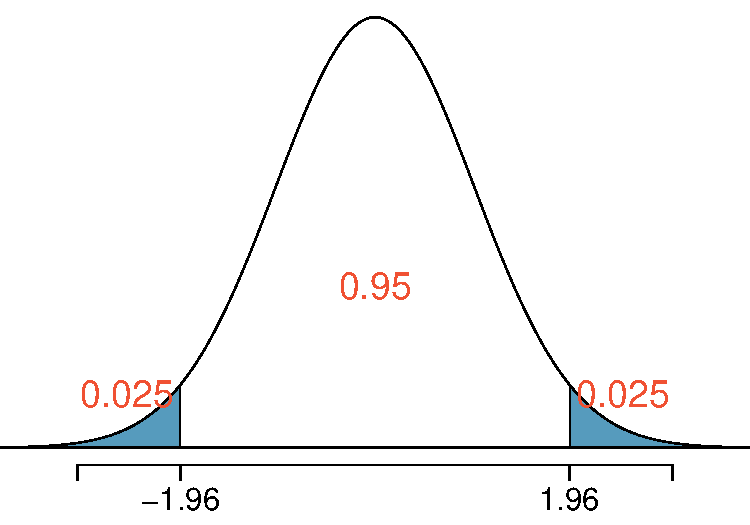
\includegraphics[width=\textwidth]{figures/sig_conf_equiv/CL95_twosided} \\
95\% confidence level \\
is equivalent to \\
two sided HT with $\alpha = 0.05$
\end{center}
}
{\pause
\begin{center}
One sided\\
~\\
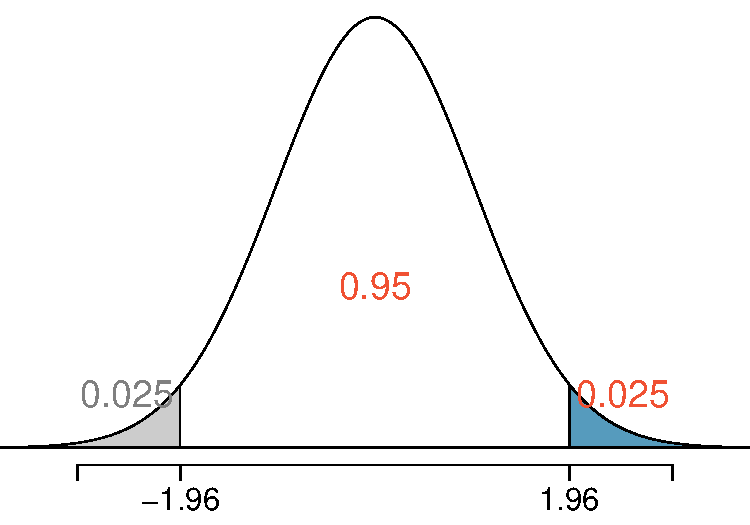
\includegraphics[width=\textwidth]{figures/sig_conf_equiv/CL95_onesided} \\
95\% confidence level \\
is equivalent to \\
one sided HT with $\alpha = 0.025$
\end{center}
}

\end{frame}

%%%%%%%%%%%%%%%%%%%%%%%%%%%%%%%%%%%%

\begin{frame}
\frametitle{}

\clicker{What is the confidence level for a confidence interval that is equivalent
to a two-sided hypothesis test at the 1\% significance level? 
\textit{Hint: Draw a picture and mark the confidence level in the center.}}

\begin{enumerate}[(a)]
\item 0.80
\item 0.90
\item 0.95
\item 0.98
\item \solnMult{0.99}
\end{enumerate}

\end{frame}

%%%%%%%%%%%%%%%%%%%%%%%%%%%%%%%%%%%%

\begin{frame}
\frametitle{}

\clicker{What is the confidence level for a confidence interval that is equivalent
to a one-sided hypothesis test at the 1\% significance level? 
\textit{Hint: Draw a picture and mark the confidence level in the center.}}

\begin{enumerate}[(a)]
\item 0.80
\item 0.90
\item 0.95
\item \solnMult{0.98}
\item 0.99
\end{enumerate}

\end{frame}

%%%%%%%%%%%%%%%%%%%%%%%%%%%%%%%%%%%%

\begin{frame}
\frametitle{}

\clicker{A 95\% confidence interval for the average normal body temperature of humans is 
found to be (98.1 F, 98.4 F). Which of the following is \emph{true}?}

\begin{enumerate}[(a)]
\item The hypothesis $H_0: \mu = 98.2$ would be rejected at $\alpha = 0.05$ in favor of $H_A: \mu \ne 98.2$.
\item The hypothesis $H_0: \mu = 98.2$ would be rejected at $\alpha = 0.025$ in favor of $H_A: \mu > 98.2$.
\item \solnMult{The hypothesis $H_0: \mu = 98$ would be rejected using a 90\% confidence interval.}
\item \solnMult{The hypothesis $H_0: \mu = 98.2$ would be rejected using a 99\% confidence interval.}
\end{enumerate}

\end{frame}

%%%%%%%%%%%%%%%%%%%%%%%%%%%%%%%%%%%%

\subsection{Results that are statistically significant are not necessarily practically significant}
\label{mi3}

%%%%%%%%%%%%%%%%%%%%%%%%%%%%%%%%%%%%

\begin{frame}
\frametitle{3. Results that are statistically significant are not necessarily practically significant}

\clicker{All else held equal, will p-value be lower if $n = 100$ or $n = 10,000$?}

\begin{enumerate}[(a)]
\item $n = 100$
\item \solnMult{$n = 10,000$}
\end{enumerate}

\soln{\pause \pause
Suppose $\bar{x} = 5$, $s = 2$, $H_0: \mu = 4.5$, and $H_A: \mu \ge 4.5$.\\
\pause
{\small
\begin{eqnarray*}
Z_{n = 100} &=& \frac{5 - 4.5}{\frac{2}{\sqrt{100}}} \pause = \frac{5 - 4.5}{\frac{2}{10}} = \frac{0.5}{0.2} = 2.5,~~~\text{p-value} = 0.0062 \\
\pause
Z_{n = 10000} &=& \frac{5 - 4.5}{\frac{2}{\sqrt{10000}}} \pause = \frac{5 - 4.5}{\frac{2}{100}} = \frac{0.5}{0.02} = 25,~~~\text{p-value} \approx 0
\end{eqnarray*}
}
\pause
\begin{center}
As $n$ increases - $SE$ $\downarrow$, $Z$ $\uparrow$, p-value $\downarrow$
\end{center}
}

\end{frame}

%%%%%%%%%%%%%%%%%%%%%%%%%%%%%%%%%%%%

\subsection{Hypothesis tests are prone to decision errors}
\label{mi4}

%%%%%%%%%%%%%%%%%%%%%%%%%%%%%%%%%%%%

\begin{frame}
\frametitle{4. Hypothesis tests are prone to decision errors}

\begin{center}
\begin{tabular}{l l | c c}
\multicolumn{2}{c}{} & \multicolumn{2}{c}{\textbf{Decision}} \\
& & fail to reject $H_0$ &  reject $H_0$ \\
  \cline{2-4}
& $H_0$ true & \onslide<3->{\green{$\checkmark$}} &  \onslide<4->{\red{Type 1 Error, $\alpha$}} \\
\raisebox{1.5ex}{\textbf{Truth}} & $H_A$ true & \onslide<5->{\red{Type 2 Error, $\beta$}} & \onslide<6->{\green{Power, $1 - \beta$}} \\
  \cline{2-4}
\end{tabular}
\end{center}

\begin{itemize}
\item \onslide<4->{A \hl{Type 1 Error} is rejecting the null hypothesis when $H_0$ is true: $\alpha$
\begin{itemize}
\item For those cases where $H_0$ is actually true, we do not want to incorrectly reject it more 
than 5\% of those times
\item Increasing $\alpha$ increases the Type 1 error rate, hence we prefer to small values of $\alpha$
\end{itemize}
}

\item \onslide<5->{A \hl{Type 2 Error} is failing to reject the null hypothesis when $H_A$ is true: $\beta$}

\item \onslide<6->{\hl{Power} is the probability of correctly rejecting $H_0$, and hence the 
complement of the probability of a Type 2 Error: $1 - \beta$}

\end{itemize}

\end{frame}

%%%%%%%%%%%%%%%%%%%%%%%%%%%%%%%%%%%%

\section{Summary}

%%%%%%%%%%%%%%%%%%%%%%%%%%%%%%%%%%%%

\begin{frame}
\frametitle{Summary of main ideas}

\vfill

\begin{enumerate}

\item \nameref{mi1}

\item \nameref{mi2}

\item \nameref{mi3}

\item \nameref{mi4}

\end{enumerate}

\vfill

\end{frame}

%%%%%%%%%%%%%%%%%%%%%%%%%%%%%%%%%%%

\end{document}